\section{Checks with GANDALF}\label{sec:numerics}

We checked the results of sections~\ref{sec:slices} to~\ref{sec:truncated} with the GANDALF code \citep[version 0.7.0;][]{Kanekar2025},
which integrates (\ref{eq:rmhd}) with the truncated Hermite hierarchy of one branch (section~\ref{sec:model}). All computations are in double precision on a CPU, and the GANDALF run uses its fourth-order Lawson--Runge--Kutta time step \citep[Lawson-RK4;][]{Lawson1967}. The box is periodic, with side length 1 and $k_1=2\pi$. As section~\ref{sec:truncated} requires, the fastest slice sets the time step: $\Delta t$ is chosen with a safety factor of one half on the smaller of the Alfv\'enic limit and $2\sqrt2/\rho$, the stability limit of RK4 on the imaginary axis, with $\rho=k_{\perp,\max}\max_j|\nabla_\perp(\Phi+su_j\Psi)|$.

\subsection{Spectral density and phase velocities}\label{num:spectrum}

\begin{figure}[t]
  \centering
  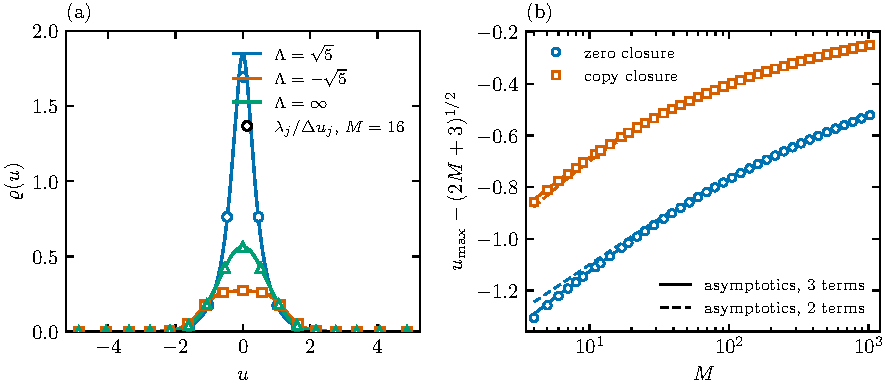
\includegraphics[width=\textwidth]{spectrum}
  \caption{(a) The spectral density $\varrho(u)$ of (\ref{eq:varrho}) for $\Lambda=\sqrt5$, $-\sqrt5$ and $\infty$ (lines), and the Gauss weights $\lambda_j$ of GANDALF's ladder matrix at $M=16$ with the zero closure, divided by the node spacing $\Delta u_j=(u_{j+1}-u_{j-1})/2$, at the nodes $u_j$ (markers in the colour of each line). (b) The largest phase velocity $u_{\max}$ of GANDALF's ladder matrix at $\Lambda=\sqrt5$, minus $(2M+3)^{1/2}$, for $M=4$ to $1024$ with the zero closure (circles) and the copy closure (squares), and the three-term (solid) and two-term (dashed) asymptotic forms (\ref{eq:umax}).}
  \label{fig:spectrum}
\end{figure}

In figure~\ref{fig:spectrum}(a), $\int\varrho\,\dd u=1/p_0$ to round-off, and by (\ref{eq:gauss}) $\lambda_j/\Delta u_j$ approximates $\varrho(u_j)$; for GANDALF's ladder matrix at $M=16$ the two differ on $|u_j|<3$ by at most 8.2\%, 1.8\% and 0.47\% for $\Lambda=\sqrt5$, $-\sqrt5$ and $\infty$. In figure~\ref{fig:spectrum}(b) the three-term forms (\ref{eq:umax}) follow the largest eigenvalue of GANDALF's ladder matrix down to $M=4$ for both closures, and it does not depend on $\Lambda$ to round-off.

\subsection{Slices in a turbulent run}\label{num:snapshots}

\begin{figure}[t]
  \centering
  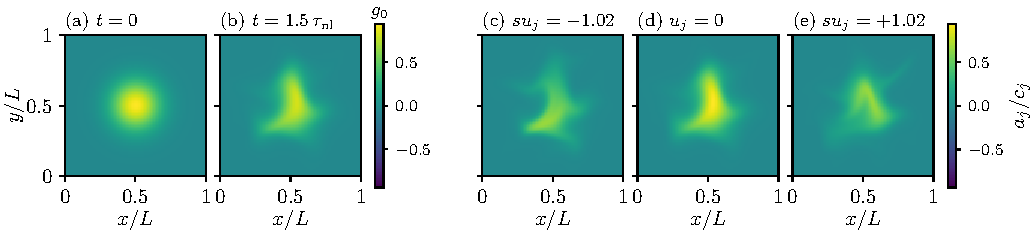
\includegraphics[width=\textwidth]{snapshots}
  \caption{A density blob in decaying Alfv\'enic turbulence, on the plane $z=0$ (coordinates in units of the box side $L=1$). (a, b) The density moment $g_0$ at $t=0$ and $t=1.5\,\tau_{\rm nl}$. (c--e) Three of the 17 slices $a_j$ of the run (section~\ref{sl:transformsec}) at $t=1.5\,\tau_{\rm nl}$, with $su_j=-1.0218$, $u_j=0$ and $su_j=+1.0218$; their stream functions $\Phi+su_j\Psi$ are mainly $z^-$, $\Phi$ alone and mainly $z^+$. At $t=0$ each slice is a constant multiple $c_jf$ of the blob $f$, and the panels show $a_j/c_j$, so all three started as panel (a). They differ at $t=1.5\,\tau_{\rm nl}$ because each was carried by its own flow, and $g_0$ in (b) is a weighted sum of all 17 slices. Panels (c) and (e) are also fainter than (d), because those slices stream along $z$ at $su_j$: the material on their plane $z=0$ started on the planes $z=+0.21$ and $z=-0.21$, where $f$ is about 0.7 of its value at $z=0$. Each group of panels has one symmetric colour scale. GANDALF run on a $64^3$ grid with $M=16$ (zero closure), $\Lambda=\sqrt5$ and $\beta_i=1$; balanced Gaussian random Elsasser fields with $1\le k_\perp/k_1\le3$ and $|k_z|/k_1\le2$, and nonlinearity parameter $\chi=\bar k_\perp z_{\rm rms}/\bar k_\parallel=1.00$, with energy-weighted mean wavenumbers $\bar k_\perp=2.45\,k_1$ and $\bar k_\parallel=1.17\,k_1$ and $z_{\rm rms}=0.478$ the rms of $|\nabla_\perp z^\pm|$; hyper-resistivity damps $z^\pm$ and every $g_m$; no forcing or hypercollisions; $f$ is a Gaussian of standard deviation $1/8$ in $x$ and $y$ and $1/4$ in $z$; $\tau_{\rm nl}=1/(\bar k_\perp z_{\rm rms})=0.1357$ is the outer eddy time.}
  \label{fig:snapshots}
\end{figure}

Figure~\ref{fig:snapshots} releases a density blob, $g(0)=f\,e_0$, into decaying Alfv\'enic turbulence with $\chi=1.00$ and follows the 17 slices of the hierarchy truncated at $M=16$. A density perturbation loads every slice with the same pattern $f$ (section~\ref{sl:forcingsec}). Each slice is then carried by its own stream function $\Phi+su_j\Psi$, which at $su_j=-1.0218$, $0$ and $+1.0218$ is mainly $z^-$, $\Phi$ alone and mainly $z^+$ (proposition~\ref{prop:elsasser}), and streams along $z$ at $su_j$. The three slices end visibly different, and $g_0$ mixes them. The slices keep their values as they are carried: on the plane $z=0$ the peaks of the slices at $su_j=\pm1.0218$ are 0.69 of the initial peak, close to the factor 0.71 by which $f$ falls over their streaming distance of 0.21 along $z$, and the peak of the slice at $u_j=0$ is 0.998 of it. GANDALF's $\partial_tg$ projected on the slices agrees with (\ref{eq:truncslice}), computed with brackets that do not use GANDALF, to $5.2\times10^{-16}$ of the largest slice rate, while the bracket term is 0.56 to 2.2 times the streaming term, and advecting every slice by $\Phi$ alone gives relative errors of 0.30 to 1.46. Over the run each slice energy changes only by the hyper-resistive loss of that slice, to $1.2\times10^{-6}$ of its initial energy, so no free energy passes between slices.

\subsection{The Hermite spectrum of decorrelated slices}\label{num:dictionary}

By section~\ref{dec:sec-dictionary}, the steady state of forced linear phase mixing is the spectrum of $\delta$-correlated slices with $e\propto\varrho$. We computed the steady state of one Fourier mode whose $g_0$ is driven by white noise from GANDALF's ladder matrix at $M=600$, with the outgoing closure $g_{M+1}=-\ii\,\mathrm{sgn}(k_z)\,g_M$ (the closure of \citealt[eq.~4.36]{Kanekar2015} with their $R_{M+1}=1$) and the Lyapunov equation for the steady covariance, and the spectrum of $\delta$-correlated slices from (\ref{eq:dictionary}) by Gauss quadrature. At $\Lambda=\infty$ the forced spectrum differs from the closed form (\ref{eq:prefactor}) by at most $3.1\times10^{-4}$, and at $\Lambda=\sqrt5$ and $-\sqrt5$ from the spectrum with $e\propto\varrho$ by at most $1.5\times10^{-4}$ and $4.2\times10^{-4}$, the size of the closure error. At $m=1$ it is 4.7\% below $(1-1/\Lambda)$ times its value at $\Lambda=\infty$ for $\Lambda=\sqrt5$ and 5.2\% above it for $\Lambda=-\sqrt5$, so this proportionality holds only at large $m$.

\subsection{Further checks and the scripts}\label{num:rhs}

The other checks cited in sections~\ref{sec:model} to~\ref{sec:truncated} use GANDALF's right-hand side. For random states with $M=2$ to 65, $\Lambda=\pm\sqrt5$ and 3, $\beta_i$ from 0.37 to 1.7 and both closures, its $\partial_tg$ satisfies (\ref{eq:truncslice}) to $2\times10^{-13}$, with brackets several times the streaming term, and fails at order one when the sign of $\{\Psi,\cdot\}$ is reversed. Slices at $su_j=-1$ obey proposition~\ref{prop:elsasser} to $5.5\times10^{-16}$ and $1.6\times10^{-15}$, and translate rigidly when $z^-=0$, to $1.4\times10^{-14}$. The two-slice law (\ref{eq:twoslice}) holds to $5\times10^{-15}$ and the two forms of (\ref{eq:fluxCD}) agree to $5\times10^{-14}$. The forms $Q^{(M)}_\varphi$ are conserved to relative rates of $3.2\times10^{-17}$, whereas $\int a_j^4\,\dd^3r$ changes at relative rates of $4.9\times10^{-4}$ and more, so only the quadratic invariants of section~\ref{sec:invariants} survive Fourier truncation.

The self-checking scripts behind these statements are in the repository \url{https://github.com/anjor/krmhd-research}, in the subfolders \url{continuum/}, \url{truncated/} and \url{dynamics/} of \url{paper/phase-velocity-slices/derivations/}; its subfolder \url{review/} holds re-derivations of the same results that share no code with them. Each script prints PASS or FAIL for every check. Figures~\ref{fig:spectrum} and~\ref{fig:snapshots} and the numbers of section~\ref{num:dictionary} come from the scripts \url{fig_spectrum.py}, \url{fig_snapshots.py} and \url{fig_dictionary.py} in \url{paper/phase-velocity-slices/analysis/}, with the configuration files in \url{paper/phase-velocity-slices/configs/}; the run of figure~\ref{fig:snapshots} is \url{P1_slices-turb_20261014_222456}, made with \url{scripts/run_slices_turbulence.py}.
